\chapter{LVM}
\label{cha:VM}



\section{Entstehung von LVM}
Unter der Bezeichnung Logical Volume Manager (LVM) existieren unter Unix Betriebsystemen verschiedene Volume Manager. Geschichtlich betrachtet wurde der erste Volume Manager unter dem Namen LVM im Jahr 1989 von IBM für deren Unix Betriebsystem AIX entwickelt. Im Jahr 1995 hat Hewlett Packard auf Basis der IBM LVM Lösung ebenfalls einen Volume Manager entwickelt.

Der Linux Logical Volume Manager wurde von Heinz Maulshagen bei der Firma Sistina entwickelt. Dieser wurde anschliessend im Februar 2000 in den Linux Kernel Release 2.3.47 aufgenommen.
Die Linux Version ist von der Bedienung her an die HP UX Version angeglichens. Die Firma Sistina hat einiges zur Storage und Clustering Fähigkeit von Linux beigetragen. Unter anderem wurde der Device-Mapper und das Global File System (GFS) von Matthew O'Keefe, welcher der Gründer von Sistina ist, entwickelt.
Es ist daher nicht weiter verwunderlich, dass die grösseren Linux Distributoren auf Sistina aufmerksam wurden. RedHat sicherte sich mit der Übernahme von Sistina im Dezember 2003 wertvolles Knowhow im Bereich Linux Storage. 

Noch unter dem Namen Sistina hat Heinz Maulshagen die zweite Version von LVM entwickelt. Dieser wurde unter dem Namen "'LVM2"' auf den Markt gebracht und war schnell von der Unix-Gemeinde wohlwollend aufgenommen worden. Im Vergleich zur Vorgängerversion ist LVM2 nicht mehr direkt in den Linux-Kernel integriert. Für eine nahtlose Integration wurde der generische Framework Device-Mapper entwickelt, welcher als Schnittstelle zum Volume Manager dient und die Block Devices verwaltet. Der Device-Mapper unterstützt den Linux Kernel ab Version 2.6 mit dem Local Volume Management. LVM2 blieb trotz dieser Architekturänderung abwärts kompatibel zu LVM, was sehr geschätzt wird. Bestehende mit dem LVM angelegten Volumes können somit mit LVM2 direkt verwaltet werden, oder können in LVM2 Volumen konveniert werden. Heute wird LVM2 mit den meisten Distributionen mitgeliefert, ist also zu einem quasi-Standard geworden. Die Enterprice Distributionen von RedHat Enterprise und Suse Enterprise Linux verwenden in der Standardkonfiguration den LVM. 

Für den Einsatz von LVM in der \gls{Cluster} Umgebung mit Shared Storage Anbindung hat RedHat die Clustering Erweiterung CLVM für LVM2 entwickelt, welche es erlaubt, den LVM Command sicher und einfach in einer Shared Storage Umgebung zu verwenden.



\section{LVM Eigenschaften}


\subsection{Architektur von LVM2}
LVM besteht aus drei Komponenten\footnote{\href{http://www.redhat.com/docs/manuals/enterprise/RHEL-5-manual/Cluster_Logical_Volume_Manager/}{http://www.redhat.com/docs/manuals/enterprise/RHEL-5-manual/Cluster\_Logical\_Volume\_Manager/}}. Die Abbildung \myref{fig:LVMMindMap} zeigt die Eigenschaften von LVM, bzw. dessen Komponenten, Befehle und Funktionen in einem Mind-Map dargestellt.

\nocite{RedHatLVM}

\begin{figure}[H]
\centering
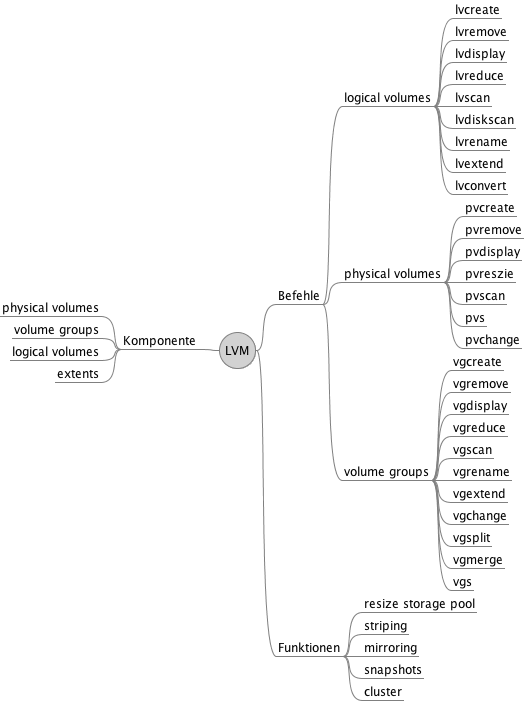
\includegraphics[width=0.75\textwidth]{LVMMindMap.png}
\caption{LVM: Mind Map}
\label{fig:LVMMindMap}
\end{figure}


\subsubsection{Physical Volumes (PV)}
Die unterste Schicht eines LVM Logical Volume ist eine physische Disk. Meist ist diese eine Festplatte, eine \gls{LUN}, welches über Storage Network \gls{SAN} zugeteilt wurde. Es kann aber auch nur eine Partition oder eine Datei sein, die als Disk verwendet wird. Eine physische Disk muss für die Verwendung im LVM als Physical Volume (PV) initialisiert werden. Dazu wird am Anfang der Disk ein entsprechender Label gesetzt, im Fachchargon auch "'labeling"' genannt.
Wie in Abbildung \myref{fig:PhysicalVolumeLayout} dargestellt, wird diese Kennzeichnung auch "'Label"' genannt, welches in den zweiten 512-Byte Sektor der Disk geschrieben wird. Dieses Kennzeichnung kann jedoch übersteuert werden, um den Label in einen der ersten Sektoren zu schreiben.

\begin{figure}[htb]
\centering
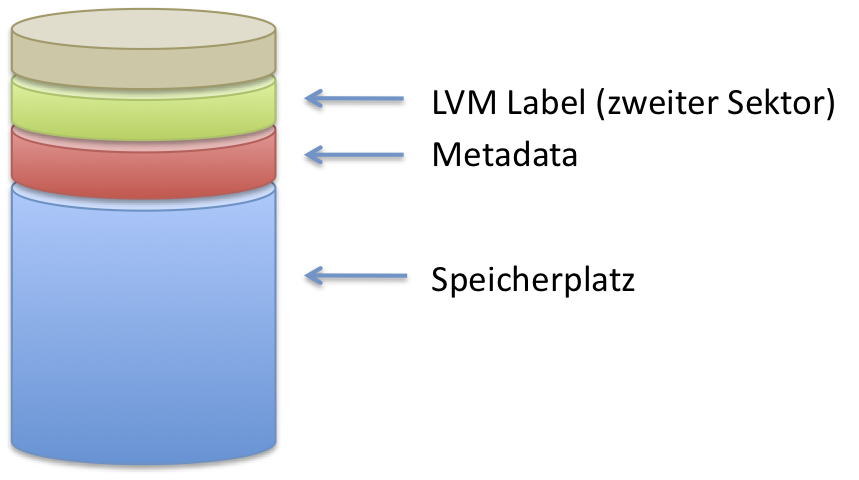
\includegraphics[width=0.8\textwidth]{PhysicalVolumeLayout.png}
\caption{Physical Volume: Layout}
\label{fig:PhysicalVolumeLayout}
\end{figure}

Der LVM Label dient dazu, die Disk korrekt zu identifizieren. Die Reihenfolge der Disk ist bei einen Neustart nicht gewährleistet, weshalb im Label ein eindeutiger zufälliger Identifikator bzw. eine Kennung, genannt "'UUID"', gespeichert wird. Anhand dieser UUID kann die Disk auch über einen Cluster wieder erkannt werden. 
Zusätzlich zur UUID sind im Label die Grösse der Disk in Bytes und die Record Adressen, in welche die LVM Metadata gespeichert sind, festgehalten.

Die LVM Metadaten enthalten die Konfigurationsdatei von LVM Volume Groups des Systems.

\subsubsection{Volume Group (VG)}\label{Volume Group (VG)}
Die Physical Volumes werden bei LVM zu Volume Groups kombiniert. Die erstellten Volume Groups dienen als Pool von Diskdpeicherplatz, welche zu Logical Volumes alloziert werden können. 
Beim Erstellen eines Volume Group aus ein oder mehreren Physical Volumes wird der Diskspeicherplatz des Physical Volumes in Einheiten bestehend aus einer fixen Grösse unterteilt, die sogenannten Physical Extents (PE).
Extents sind die kleinste physikalische Speichereinheit in einem LVM System. Die Extentsgrösse kann beim Erstellen des Volume Group gestgelegt werden, oder den Standardwert von 4 Megabyte übernommen werden. Die maximale Grösse eines Extent ist 1 Gigabyte. Die Anzahl an Extents in einer Volume Group ergibt sich aus der Summe aller Physical Volumes in einer Volume Group. Extents dienen zur "'n to m"' (Physical-to-Logical) Volumenzuordnung. Mehr dazu wird im Abschnitt \myref{Logical Volumes (LV)} erläutert.

\begin{figure}[htb]
\centering
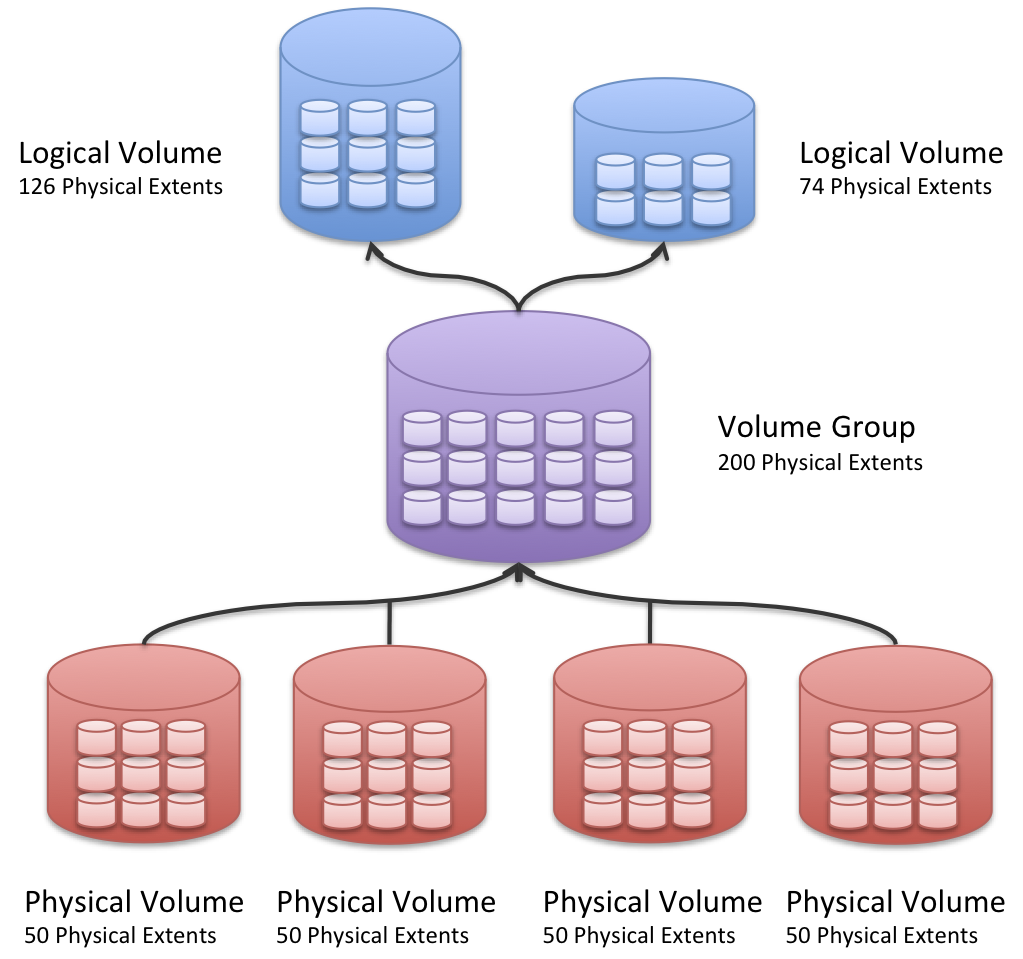
\includegraphics[width=1\textwidth]{ExtentsMapping.png}
\caption{Extents Mapping: Layout}
\label{fig:ExtentsMappingLayout}
\end{figure}

\subsubsection{Logical Volumes (LV)}\label{Logical Volumes (LV)}
Wie bereits beschrieben werden Logical Volumes aus einer Volume Group erstellt. Eine Volume Group kann in mehrere Logical Volumes unterteilt werden, jedoch kann sich ein Logical Volume nicht über mehrere Volume Groups erstrecken.
Wie im Abschnitt Volume Groups erwähnt, dienen Extents zum Zuordnen von Physical-to-Logical Volumes. Ein solches Mapping wird in Abbildung \myref{fig:ExtentsMappingLayout} veranschaulicht.
Eine Logical Volume wird analog zum Physical Volume in Extents unterteilt, sogenannte Logical Extents (LE).
Die Logical Extents besitzen die gleiche Grösse wie die Physical Extents der Volume Groups, in welcher sich das Logical Volume befindet. Die Grösse des Logical Volume setzt sich aus den Anzahl Physical Extents zusammen, welche aus der Volume Groups hinzugefügt wurde. Wird beim Erstellen der Volume Groups eine Extentgrösse von 32 Megabyte gewählt, kann die Logical Volume Grösse nur eine Vielfaches von 32 Megabyte sein. Ein Volume kann auf einen 64bit maximal 8 Exabytes gross sein. 

Die Abbildung \myref{fig:ExtentsMappingLayout} zeigt eine LVM Beispielkonfiguration. In diesem Beispiel wurden 4 Physical Volume mit je 50 Extents einer Volume Group zugeordnet. Somit verfügt die Volume Group über 200 Extents (4x50), welche sie ihren Logical Volumes zur Verfügung stellen kann. Aus diesen 200 Extents wurden in diesen Beispiel zwei Logical Volumes mit 126 Extents und 74 Extents erstellt. 

\paragraph{Flexible Kapazität} $\;$\\
Bei traditionellen Volumes kann ein Volume maximal die Grösse eines physischen Disks annehmen. Ein Logical Volume hingegen kann durch die Abstraktion fast beliebig vergrössert werden.
Durch die Zuordnung von weiteren Extents, welche in der Volume Group als "'frei"' makiert sind, kann das Logical Volume vergrössert werden. Wächst der Speicherplatz eines der beiden Logical Volumes gemäss Abbildung  \myref{fig:ExtentsMappingLayout}, müsste die Volume Group mit einer oder mehreren zusätzlichen Physical Volume ergänzt werden, um der Logical Volumes mehr Extents zuordnen zu können.

Umgekehrt kann das Logical Volume durch das Entfernen von Extents verkleinert werden. Sind in der Volume Group keine freien Extents mehr verfügbar, kann die Volume Group durch Zuordnung von weiteren Physical Volume vergrössert werden, welche wiederum einer Logical Volume Group zugeordnet werden kann.
Die kleinstmöglichste Wachstumgrösse der Logical Volume ist eine Extentsgrösse. Mehr zur Extentsgrösse wird im Abschnitt \myref{Volume Group (VG)} erklärt. 

\paragraph{Unterbruchsfreie Umplatzierung der Daten} $\;$\\
Durch LVM können die Logical Volumes inkl. Dateisystem und deren Daten zur Laufzeit auf neuere, performantere Speichersysteme umplatziert werden, ohne deswegen den Betrieb unterbrechen zu müssen. Trotz Verwendung der Disks ist es möglich, die Daten im Volume neu zu organisieren. Somit ist es kein Problem, eine verwendete physische Disk von Daten zu befreien, bevor diese ersetzt bzw. entfernt wird (z. B. bei der Renovation der physischen Umgebung).


\paragraph{Striping Volume} $\;$\\
Bei hoher Anzahl von sequenziellen schreib und lese zugriffe auf eine Volume ist es empfehlenswert eine Strips Volume zu verwenden. Striped Volumes 


\paragraph{Spiegelung von Volumes (Mirroring)} $\;$\\
Mirrored Logical Volumes sind exakte Kopien eines Volumes, welche durch Spiegelung, auch Mirroring genannt, dauernd mit dem Original in Synchronisation gehalten werden.
Wenn bei einem LVM für ein Volume eine Mirrored Logical Volume erstellt wird, stellt LVM sicher, dass wenn Daten auf ein darunter liegendes Physical Volume geschrieben werden soll, die Daten automatisch auf ein weiteres Physical Volume gespiegelt werden. LVM unterstützt zudem das Spiegeln auf mehrere Mirrored Volume. Durch die redundante Speicherung der Daten auf verschiedene Physical Volumes, werden die Daten und das System von Diskfehler besser geschützt. Tritt der Fall eines physischen Diskdefekt ein, steht zwar dieses Laufwerk dem System nicht mehr zur Verfügung, erlaubt aber dem System ohne Unterbruch mit den zusätzlichen Mirrored Volumes weiterzuarbeiten.
Für das Mirroring wird das Physical Volume in Regionen unterteilt, der Standardwert für die Region-Grösse ist 512 KB, zusätzlich wird ein kleines Log geführt, um nachzuvollziehen, welche Regionen deckungsgleich mit dem Original sind. Das Log wird zumeist aus Sicherheitsgründen auf eine weitere Disk bzw. Volume abgelegt. Manchmal wird es im Memory geführt, was aber bei einem Systemabsturz gefährliche Nachteile in sich birgt.

\begin{figure}[H]
\centering
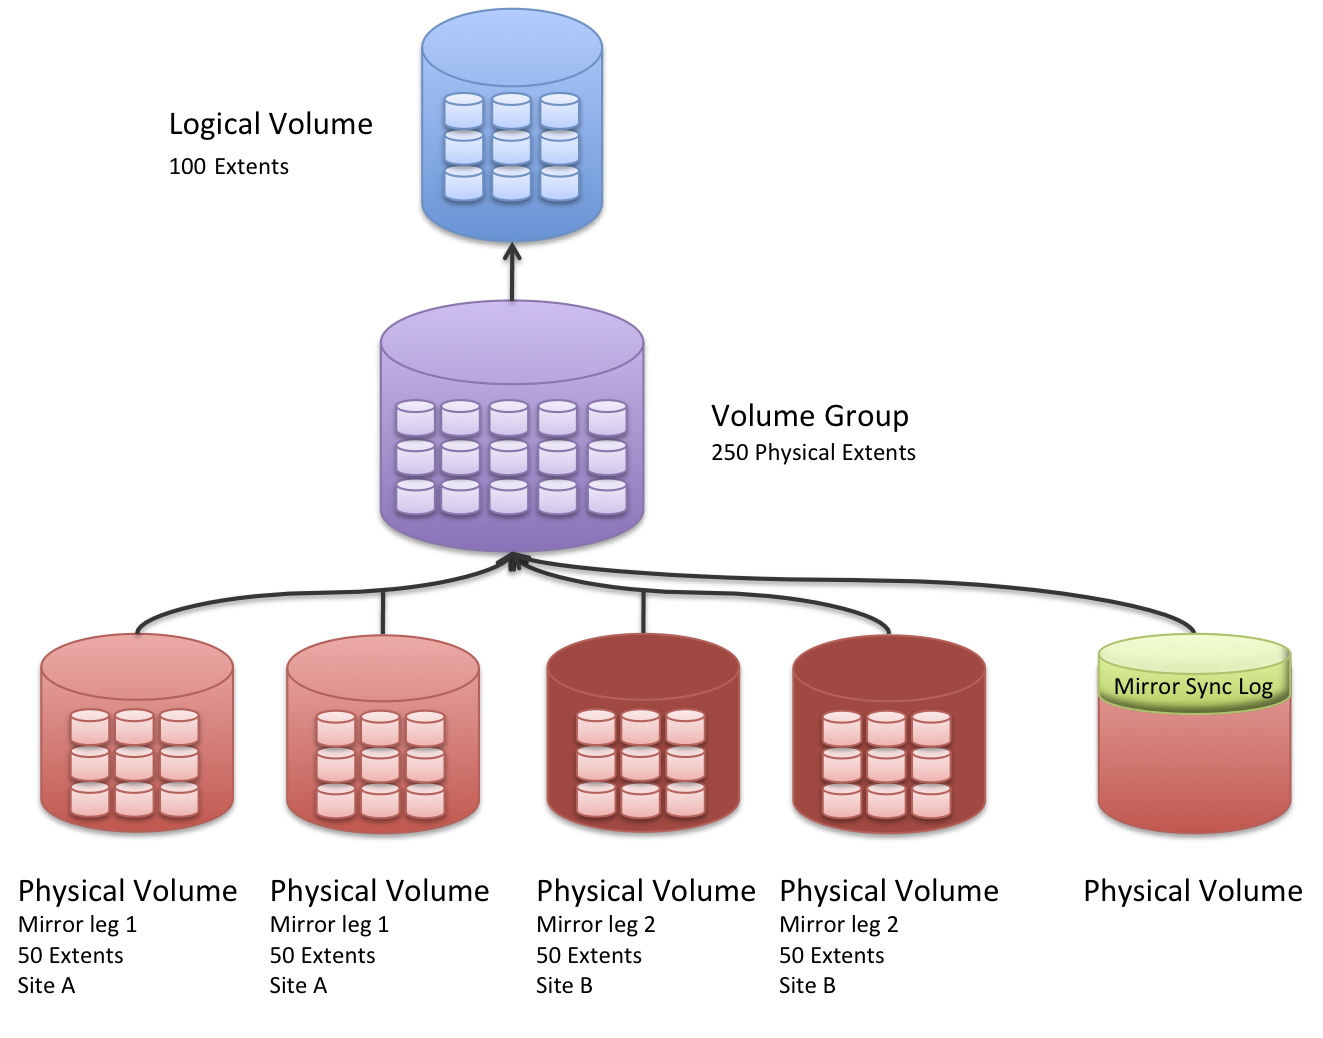
\includegraphics[width=1\textwidth]{LVMMirrorArchitectur.png}
\caption{LVM: Mirror Architektur}
\label{fig:LVM Mirror Architektur}
\end{figure}

Mirroring wird in den meisten Fällen nicht als Ersatz eines RAID-1 Systeme betrachtet. In vielen Modernen IT-Landschaften werden die Disk bzw. \gls{LUN} über eine Storage Area Network (\gls{SAN}) einem System zur Verfügung gestellt. Diese \gls{LUN} stammen meist aus einer RAID-1 oder RAID-5 Diskgruppe und sind somit im Storage System redundand. Das Mirroring wird in solchen Fällen meist zur Spiegelung der Daten in ein weiteres Rechenzentrum angewendet. Indem das LVM mehrere mirrored Disks unterstützt, können die Daten in mehrere Rechenzentren gespiegelt werden. 


Die Abbildung \myref{fig:LVM Mirror Architektur} zeigt eine mögliche Architektur eines LVM Mirrors, welche über zwei Rechenzentren Site A und Site B gespiegelt wird. Dazu wurden je zwei Physical Volume über jeweils eine Network Storage System pro Rechenzentrum zugeordnet. Das Mirror Log wird auf eine separaten Physical Volume geschrieben. Mit dieser Architektur lassen sich in Cluster Umgebungen hoch redundante Systeme bauen.


\paragraph{Snapshot} $\;$\\
LVM unterstützt das Erstellen von \gls{Snapshot}s eines Logical Volume. Wenn ein \gls{Snapshot} erstellt wurde, werden alle Änderungen im Volume im \gls{Snapshot} gespeichert und das Original Volume bleibt unverändert im Originalzustand. Beim Erstellen eines \gls{Snapshot} ist darauf zu achten, dass die Snapshot-Grösse etwas mehr Speicherplatz zur Verfügung steht, als die geplante Änderung benötigt. Sobald der reservierte Speicherplatz eines \gls{Snapshot} voll ausgenutzt wurde, können neue Änderungen nicht mehr nachvollzogen bzw. gespeichert werden, wodurch das \gls{Snapshot} ungültig wird und alle Änderungen verloren gehen.
Um ein "'Überlaufen"' zu verhindern, sollten \gls{Snapshot} regelmässig und zeitnah überwacht werden und bei Bedarf genügend vergrössert werden.

Snapshots bieten beim Betrieb eines Systems einige Vorteile:

\begin{figure}[htb]
\centering
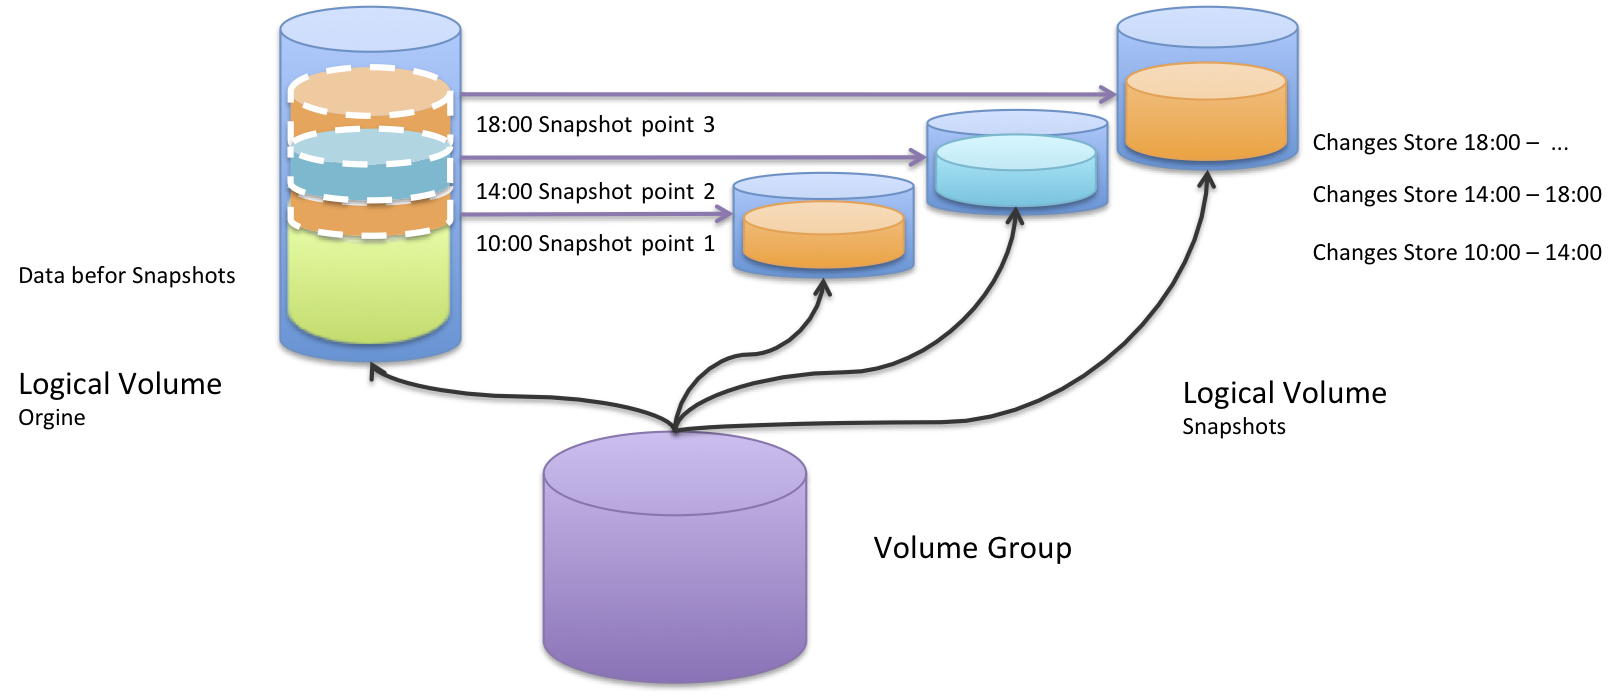
\includegraphics[width=1.2\textwidth]{LVMSnapshot2.png}
\caption{LVM: Snapshot}
\label{fig:LVMSnapshot}
\end{figure}


\begin{itemize}
\item Es können Tests gegen produktive Daten durchgeführt werden
\item Sollen z.B. Datenbanken während des laufenden Betriebes gesichert werden, können mit Hilfe der LVM \gls{Snapshot} Technologie die Daten parallel gesichert werden, auch wenn zur gleichen Zeit die Originaldaten (zu sichernde Daten) sich verändern sollten (erhalten der Datenkonsistenz).
\item Ein File-Systemcheck kann mit Hilfe der LVM Technologie auf dem Filesystem getestet werden.
\end{itemize}

\paragraph{Clustered Logical Volume Manager} $\;$\\
Clustered Logical Volume Manager (CLVM) ermöglicht es, wie im Abschnitt "'Entstehung LVM"' erwähnt, die Verwendung von LVM im \gls{Cluster} Umfeld. CLVM besteht aus dem Deamon clvmd welche auf allen \gls{ClusterNode}s installiert und während des Bootvorgangs gestartet sein müssen. Bei einer Änderung an der Volume Konfiguration verteilt der Deamon clvmd die aktuellen LVM Metadaten an alle Nodes und ermöglicht damit, dass alle Nodes dieselbe Sicht auf die Logical Volumes haben. In der Konfigurations Datei  lvm.conf von LVM muss für CLVM der Locking Typ der Volumes auf Typ 3 "'Built-in clustered locking"' angepasst werden.


\section{Einarbeiten in LVM (LVM2 Commands)}

\subsection{Physical Volume anlegen}

Mit folgendem Beispielbefehl werden aus einem Block-Laufwerk \textit{/dev/sdb}, \textit{/dev/sdc}, \textit{/dev/sdd} und \textit{/dev/sde} vier Physical Volumes erstellt und gelabelt.  

\Shell{pvcreate /dev/sdb /dev/sdc /dev/sdd /dev/sde}


Mehr Informationen sind in den MAN Pages\footnote{\href{http://linux.die.net/man/8/pvcreate}{http://linux.die.net/man/8/pvcreate}}  zu finden.

\subsection{Physical Volume entfernen}

Mit dem Befehl  \textbf{pvremove} kann ein Physical Volume Label auf aus einem Block-Laufwerk entfernt werden.

\Shell{pvremove /dev/sdb}


Mehr Informationen sind in den MAN Pages\footnote{\href{http://linux.die.net/man/8/pvcreate}{http://linux.die.net/man/8/pvcreate}}  zu finden.

\subsubsection{Volume Group anlegen}

Mit dem Befehl vgcreate kann man aus einem oder mehreren Physical Volumes eine Volume Group erstellen. Die Extentsgrösse kann mit der Option \textbf{-s} bestimmt werden. Wird diese Option nicht genutzt, so verwendet das LVM die Standardgrösse, welche in der lvm.conf festgelegt ist. Die Extentgrösse von 32 MB hat sich in der Praxis bewährt.
Grössere Extents haben keinen Einfluss auf eine verbesserte I/O Performance.
Die Zuordnung der Physical Extents, kann mit \textbf{--alloc} definiert werden. Die Standardkonfiguration \textbf{normanl} muss nur in speziellen Fällen angepasst werden, wenn aus speziellen Performancegründen evtl. beim Backup parallele Strips gewünscht wird.

\Shell{vgcreate VolGroupData}

Volume Groups in einer Cluster-Umgebung, welche mit CLVM auf einem geteilten Storage erstellt wurden, sind von allen Cluster Nodes sichtbar. Mit der Option \textbf{-c} wird die Sichtbarkeit der Volume Group auf den lokalen Node beschränkt.

\Shell{vgcreate -c VolGroupCluData1 /dev/sdb /dev/sdc /dev/sdd /dev/sde}


Mehr Informationen sind in den MAN Pages\footnote{\href{http://linux.die.net/man/8/vgcreate}{http://linux.die.net/man/8/vgcreate}} zu finden.

\subsubsection{Konfiguration von Volume Group auslesen}

Mit dem Befehl \textbf{vgdisplay} \textbf{vgs} kann die Konfiguration der Volume Group ausgelesen werden.
Der Befehl \textbf{vgdisplay} eignet sich um eine schnelle Übersicht zu gewinnen. Der Befehl \textbf{vgs} eignet zum Auslesen der Konfiguration per Script, da mit Optionen die Ausgabe individuell angepasst werden kann.

\Shell{vgdisplay VolGroupCluData1}

\Shell{vgs}


Mehr Informationen sind in den MAN Pages\footnote{\href{http://linux.die.net/man/8/vgdisplay}{http://linux.die.net/man/8/vgdisplay}} \footnote{\href{http://linux.die.net/man/8/vgs}{http://linux.die.net/man/8/vgs}} zu finden.

\subsubsection{Konfiguration von Volume Group anpassen}

Mit dem Befehl \textbf{vgchange} kann die Konfiguration einer bestehende Volume Group angepasst werden.


Mehr Informationen sind in den MAN Pages\footnote{\href{http://linux.die.net/man/8/vgchange}{http://linux.die.net/man/8/vgchange}} zu finden.

\subsubsection{Volume Group vergrössern}

Durch Hinzufügen von weiteren Physical Volumes kann eine Volume Group vergrössert werden und somit Speicherplatz für weitere Logical Volumes oder vergrösserte Logical Volumes zur Verfügung gestellt werden.

\Shell{vgextent VolGroupCluData1  /dev/sdf /dev/sdg }


Mehr Informationen sind in den MAN Pages\footnote{\href{http://linux.die.net/man/8/vgextent}{http://linux.die.net/man/8/vgextent}} zu finden.

\subsubsection{Volume Group entfernen}

Sind alle Logical Volumes einer Volume Group entfernt worden, kann mit dem Befehl \textbf{vgremove} die Volume Group vom System entfernt werden. Die Eigenschaft "'Cur LV"' der Ausgabe von \textbf{vgdisplay} zeigt die Anzahl Logical Volumes der Volume Groupe und sollte vor dem Entfernen der Volume Group 0 stehen.

\Shell{vgremove VolGroupCluData1}

Mehr Informationen sind in den MAN Pages\footnote{\href{http://linux.die.net/man/8/vgremove}{http://linux.die.net/man/8/vgremove}} zu finden.

\subsubsection{Logical Volume anlegen}

Mit dem Befehl \textbf{lvcreate}  können lineare, striped oder mirrored Volumes angelegt werden.
Grundvoraussetzung für das Anlegen eines Logical Volumes ist, dass auf dem System bereits mindestens eine Volume Group angelegt wurde.

In diesen Beispiel wird eine Logical Volume mit der Grösse von 2 GB auf der Volume Groupe VolClusterData1 angelegt. 

\Shell{lvcreate -L 2G VolClusterData1}

Wird kein Namen für das Logical Volume mit der Option \textbf{-n lvname} festgelegt, vergibt LVM automatisch einen generierten Namen "'lvol0"' (dieser wird durchnummeriert).

\Shell{lvcreate -L 2G VolClusterData1 -n clvdata1}

Die Grösse eines LVM kann auch prozentual zur Volume Group Grösse mit dem Zusatz \textbf{VG} definiert werden oder prozentual zum restlichen freien Speicherplatz der Volume Group mit dem Zusatz \textbf{FREE}.

\Shell{lvcreate -L 50\%VG VolClusterData1 -n clvdata1}

\Shell{lvcreate -L 50\%FREE VolClusterData1 -n clvdata1}

Mehr Informationen sind in den MAN Pages\footnote{\href{http://linux.die.net/man/8/lvcreate}{http://linux.die.net/man/8/lvcreate}}  zu finden.

\subsubsection{Striped Locical Volume anlegen}

Eine Striped Logical Volume wird mit \textbf{lvcreate} und der Option \textbf{-i} und der Anzahl an Physical Volumes aus der Volume Group angelegt, welche für LVM verwendet werden soll. Die Grösse eines einzelnen Strips kann mit der Option \textbf{-I} festgelegt werden. In der Praxis haben sich Stripgrössen von 64kB oder 128kB bewährt.

\Shell{lvcreate -L 2G  -i2 -I64 VolClusterData1 -n clvdata1}

\subsubsection{Mirrored Locical Volume anlegen}

Eine Mirrored Logical Volume wird mit der Option \textbf{-m} plus der Anzahl der Mirrored Volumes angelegt. Das unten aufgeführte Beispiel legt zwei Mirrored Volumes an und legt somit fest, dass die Daten dreifach gespeichert werden sollen.

\Shell{lvcreate -L 2G -m2 VolClusterData1 -n clvdata1}


\subsubsection{Logical Volume grösse anpassen}

Wird mehr Speicherplatz im Logical Volume benötigt, kann der Speicherplatz mit dem Befehl \textbf{lvresize} 
angepasst werden. Bevor man das Logical Volume vergrössert, sollte man prüfen, ob die darunter liegende Volume Groupe noch genügen freie Extents hat.

\Shell{lvextend -L +2G /dev/VolGroupCluData1/VolClusterData1 }

Eine Logical Volume kann auf dieselbe Weise auch wieder verkleinert werden. Hier ist darauf zu achten, dass man das darüber liegende Filessystem vorher verkleinert hat.

\Shell{lvextend -L -1G /dev/VolGroupCluData1/VolClusterData1 }

Mehr Informationen sind in den MAN Pages\footnote{\href{http://linux.die.net/man/8/lvextend}{http://linux.die.net/man/8/lvextend}} zu finden.

\subsubsection{Logical Volume entfernen}

Wird das Logical Volume nicht mehr benötigt, kann das Logical Volume mit dem Befehl \textbf{lvremove} 
entfernt werden. Die Verwendeten Extents des Logical Volume werden in der Volume Group als frei markiert. Achtung alle Daten auf dem Volume gehen verloren. 

\Shell{lvremove /dev/VolGroupCluData1/VolClusterData1 }

Mehr Informationen sind in den MAN Pages\footnote{\href{http://linux.die.net/man/8/lvremove}{http://linux.die.net/man/8/lvremove}} zu finden.
